\documentclass[Protokollheft.tex]{subfiles}
\begin{document}
\chapter{HF-Zeitbereich 3: Streuparameter}
%--------------- Start Vorbereitungsaufgaben ---------------
Dieser Versuch schließt direkt an den letzten Versuch an. Es soll dieselbe
Problemstellung sowie das im letzten Versuch bestimmte Zeitsignal verwendet werden,
um dann mithilfe der DFT Analysen im Frequenzbereich durchzuführen. Insbesondere 
werden die Anregung $I_0$ sowie die Abschlusswiderstände wieder über die jeweilige 
Stirnfläche verteilt. Beachten Sie aber, dass im Gegensatz zum letzten Versuch hier nun
für die homogene Leitung eine relative Permittivität von $\epsr=0.9$ verwendet wird.
Dieser Wert ist zwar unphysikalisch, stellt aber sicher, dass der 
Leitungswellenwiderstand \SI{50}{\ohm} beträgt. Für die inhomogene Leitung gilt weiterhin
$\epsr=1.3$, während für beide Leitungen weiterhin $\mur=1$ gewählt wurde.

\section{Vorbereitungsaufgaben}

% --> Aufgabe
\begin{framed}
	\noindent \textbf{1.} Zeichnen Sie für die hier behandelte Leitung das entsprechende Zweitor mit Zählpfeilen orientiert wie in Abb.~7.7. Fügen Sie auch die hier verwendete äußere Beschaltung an den Leitungsenden hinzu.\label{exer:twoPort}
\end{framed}

\begin{figure}[h]
	\centering
	\def\svgwidth{0.8\textwidth}
	\input{schaltung.pdf_tex}
	\caption{Zweitor}
	\label{fig:schal}
\end{figure}
% --> Aufgabe
\begin{framed}
	\noindent \textbf{2.} Bestimmen Sie den Eingangsstrom $I_1$ in Abhängigkeit von der Eingangsspannung $U_1$, dem Abschlusswiderstand $R$ und der Anregung $I_0$.\label{exer:calcI1}
\end{framed}

Um das Strom $I_1$ zu bestimmen, betrachtet man die Stromquelle $I_0$ und  das ersten Knoten. Aus die Knotenanalyse erhält man folgende Gelichung: 
\begin{eqnarray}
I_0  = I_1 + \frac{U_1}{R} \\
I_1 = I_0-\frac{U_1}{R}.
\end{eqnarray}
 

% --> Aufgabe
\begin{framed}
	\noindent \textbf{3.} Bestimmen Sie die Ausgangsspannung $\ul{U}_2$ und den Ausgangsstrom $\ul{I}_2$ in Abhängigkeit von der Eingangsspannung $U_1$, der Länge der Leitung $\ell$ und der Phasenkonstante $\beta$. Sie können dabei annehmen, dass die Leitung mit ihrem Wellenwiderstand abgeschlossen ist.\label{exer:calcU2I2}
\end{framed}
In dem Versuch 7 und 8 geht es um Koaxialleiter. Um die $U_2$ und $I_2$ zu finden, nutzt man schön aus Versuch 7 bekannte Leitungsgleichungen.

\begin{eqnarray}
\underline{U}(z)&=&U^{+}_0\exp(-j\beta z)+U^{-}_0\exp(+j\beta z)\\
\underline{I}(z)&=&I^{+}_0\exp(-j\beta z)-I^{-}_0\exp(+j\beta z)=\frac{U^{+}_0}{Z_w}\exp(-j\beta z)-\frac{U^{-}_0}{Z_w}\exp(+j\beta z)
\end{eqnarray}

Weil die Leitung mit einem Wellenwiderstand abgeschlossen ist, betrachtet man die rücklaufende Welle nicht.

\begin{eqnarray}
\underline{U}(z)&=&U^{+}_0\exp(-j\beta z)\\
\underline{I}(z)&=&I^{+}_0\exp(-j\beta z)=\frac{U^{+}_0}{Z_w}\exp(-j\beta z)
\end{eqnarray}
Zuerst bestimmt man $U_1$.\\
 $U_1$ befindet sich bei $\underline{U}(z=0)$ . 

$$U_1=\underline{U}(z=0)=U^{+}_0 $$

Analog zu $U_1$ bekommt man auch $\underline{U}_2$ und $\underline{I}_2 $, nur soll man als $z$ die Länge der Leitung $\ell$ einsetzen. 

\begin{eqnarray}
\underline{U}_2=\underline{U}(z=\ell)&=&U^{+}_0\exp(-j\beta \ell)\\
\underline{I}_2=-\underline{I}(z=\ell)&=&-I^{+}_0\exp(-j\beta \ell)=-\frac{U^{+}_0}{Z_w}\exp(-j\beta \ell)
\end{eqnarray}
Am Ende bekommt man

$$\underline{U}_2=U_1\exp(-j\beta \ell)$$
$$\underline{I}_2=-\frac{U_1}{Z_w}\exp(-j\beta \ell). $$

% --> Aufgabe
\begin{framed}
	\noindent \textbf{4.} Mit welcher Geschwindigkeit bewegt sich die Welle auf der gegebenen Leitung? Berechnen Sie die Zeit, die die Welle benötigt, um die Länge der Leitung einmal zu passieren.\label{exer:calcSpeedTime}
\end{framed}
\noindent
Für die Ausbreitungsgeschwindigkeit $c$ eines Elektrischen Impulses in einem Material gilt 
\begin{equation}
 \label{eq:cSpeed}
 c = \frac{1}{\sqrt{\mu \varepsilon}}
\end{equation}.\\
Damit ergibt sich für den homogenen Leiter mit $\mu_r = 1$ und $\varepsilon_r = 0.9$ eine Ausbreitungsgeschwindigkeit von $3.16 \cdot 10^8 \ \si{ \frac{m}{s}}$ womit die Leitung in $4.75\cdot 10^{-9} \  \si{ s} = 4.75 \  \si{ ns}$ passiert wird. \\
Für die inhomogene Leitung mit $\varepsilon_r = 1.3$ für den Anfang und das Ende und $\varepsilon_r = 10$ für die Inhomogenität, ergibt sich durch aufspalten eine Ausbreitungsgeschwindigkeit von $2.63\cdot 10^8 \ \si{\frac{m}{s}}$ im Anfang und Ende und $ 9.48 \cdot 10^7 \ \si{\frac{m}{s}}$ in der Inhomogenität. Hiermit ergibt sich eine Passierdauer von $1.58\cdot 10^{-8} \ \si{s} = 15.8 \ \si{ns}$.

% --> Aufgabe
\begin{framed}
	\noindent \textbf{5.} Wie kann man aus den im Allgemeinen komplexen Rückgabewerten der DFT (\matlab-Befehl \verb"fft") auf das Frequenzspektrum schließen?\label{exer:freqSpectByDFT}
\end{framed}
\noindent
Um aus den Rückgabewerten der DFT ein Frequenzspektrum zu erstellen müssen die Frequenzpunkte gleichmäßig aufgetragen werden und anschließend darüber die, durch die Anzahl der Sampels geteilten, Rückgabewerte der DFT aufgetragen werden. 

\section{Aufgaben während der Praktikumssitzung}

{\subsection{Streuparameter}}

\noindent
Im Folgenden soll das Übertragungsverhalten der beiden Leitungen
im Frequenzbereich von $0$ bis \SI{200}{MHz} bestimmt werden. Zu diesem
Zweck sollen nur noch Gaußpulse verwendet werden.

% --> Aufgabe
\begin{framed}
	\noindent \textbf{1.} Regen Sie die homogene Leitung mit dem in Versuch 7 beschriebenen
Gauß-Puls an.\label{exer:exciteGauss}
\end{framed}
% --> Aufgabe
\begin{framed}
	\noindent \textbf{2.} Bestimmen Sie die Spannungen und Ströme an Ein- und Ausgang der Leitung
 im Zeitbereich und stellen Sie diese in entsprechenden Plots dar.\label{exer:UandVtimeDomain}
\end{framed}
\noindent
\begin{figure}
	\centering
	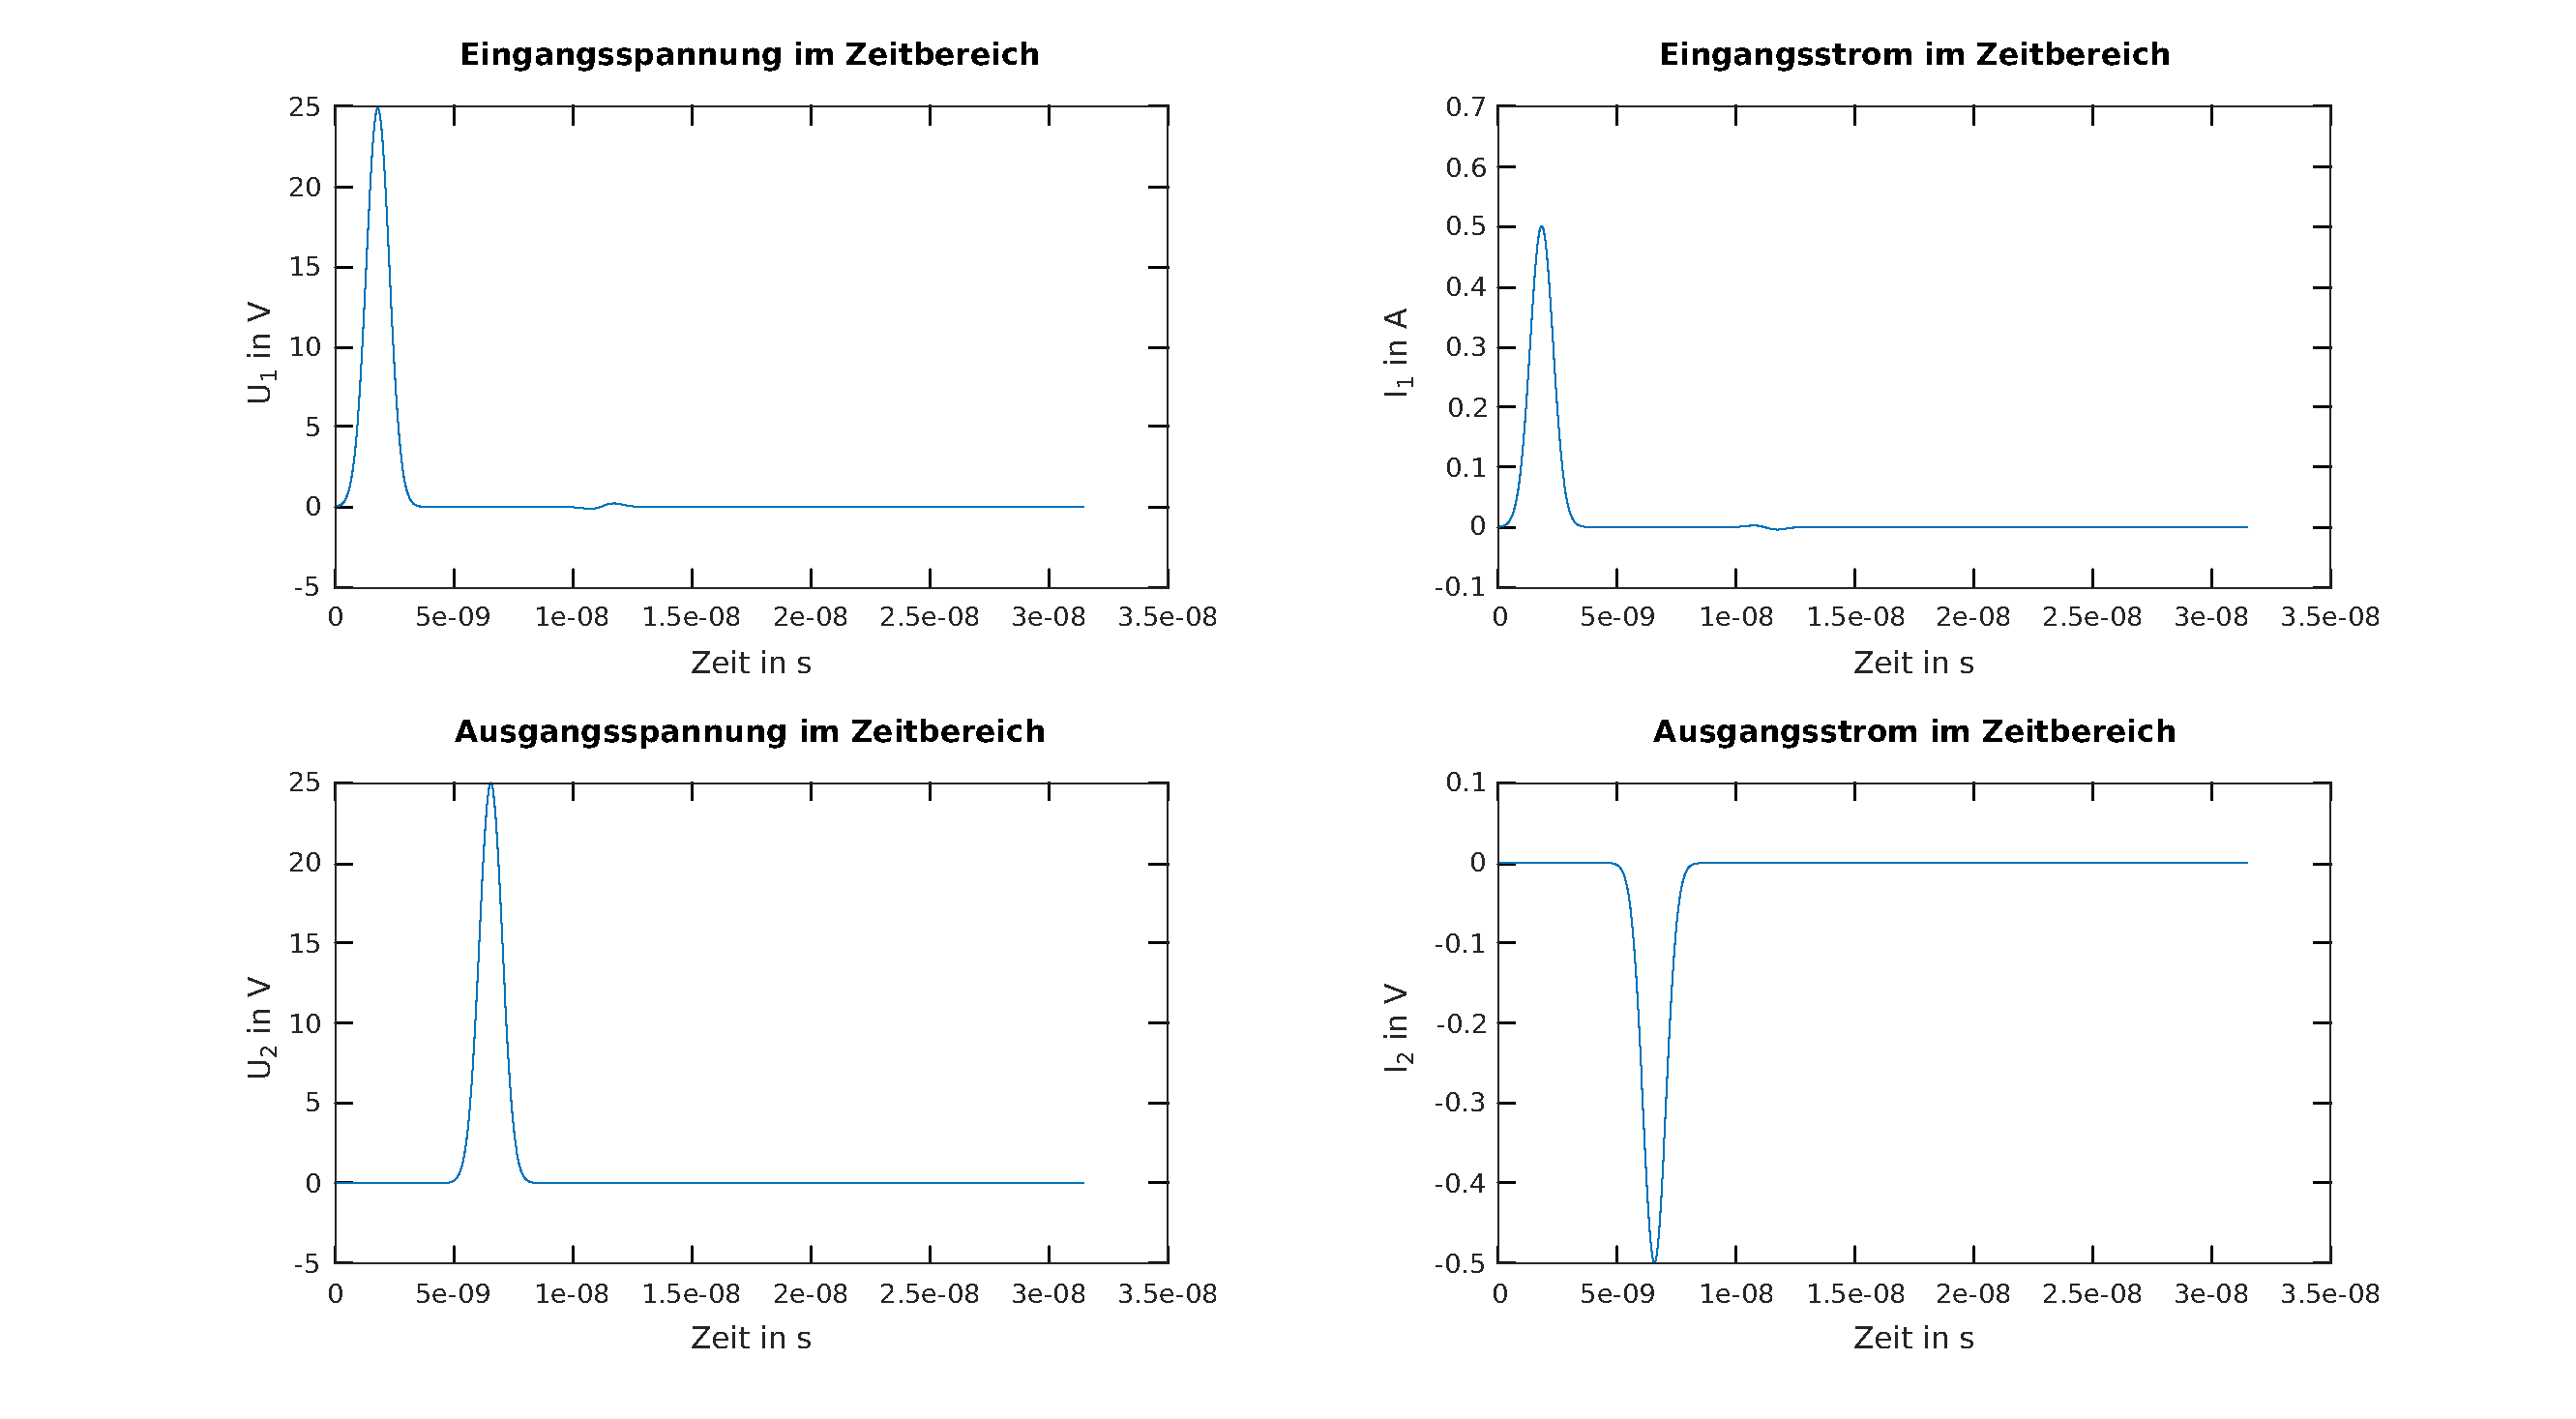
\includegraphics[width=0.9\linewidth]{EinAusSpanStromZeit}
	\caption{Ein- und Ausgangsspannungen  und Ströme der homogenen Koaxialleitung im Zeitbereich}
	\label{fig:einausspanstromzeit}
\end{figure}
Wie in Abb. \ref{fig:einausspanstromzeit} zu erkennen wird ein Gaussimpuls in die Leitung eingespeist, der mit einer geringen Verzögerung von ca. $0.5\cdot 10^-8 \ \si{s}$  am Ende ankommt. Die Der Ausgangsstrom ist aufgrund der Wahl der Flussrichtungen dem Eingangstrom mathematisch entgegen gerichtet.  
% --> Aufgabe
\begin{framed}
	\noindent \textbf{3.} Schreiben Sie eine Routine, die das Spektrum eines
Zeitsignals berechnet und eine zugehörige Frequenzachse erzeugt.
Experimentieren Sie mit dem zero-padding, um im interessierenden
Frequenzbereich eine genügend gute Auflösung zu bekommen.\label{exer:calcFreqSpectWithAxis}
\end{framed}
% --> Aufgabe
\begin{framed}
	\noindent \textbf{4.} Bestimmen Sie die Spannungen und Ströme an Ein- und Ausgang der Leitung 
im Frequenzbereich und stellen Sie diese in entsprechenden Plots dar. Überprüfen Sie, ob 
der Gauß-Puls im Frequenzbereich die Bedingungen erfüllt, die an 
diesen in Versuch 7 gestellt wurden.\label{exer:UandVfreqDomain}
\end{framed}
\noindent
Wie in Abb. \ref{fig:einausspanstromfrequenz} zu sehen nehmen Ein- und Ausgangsspannung sowie Strom mit zunehmender Frequenz ab. \\
Der Grußimpuls erfüllt im Frequenzbereich die Anforderung ein Begrenztes Signal zu haben, da er mit zunehmender Frequenz zu Null hin abfällt. 
\begin{figure}
	\centering
	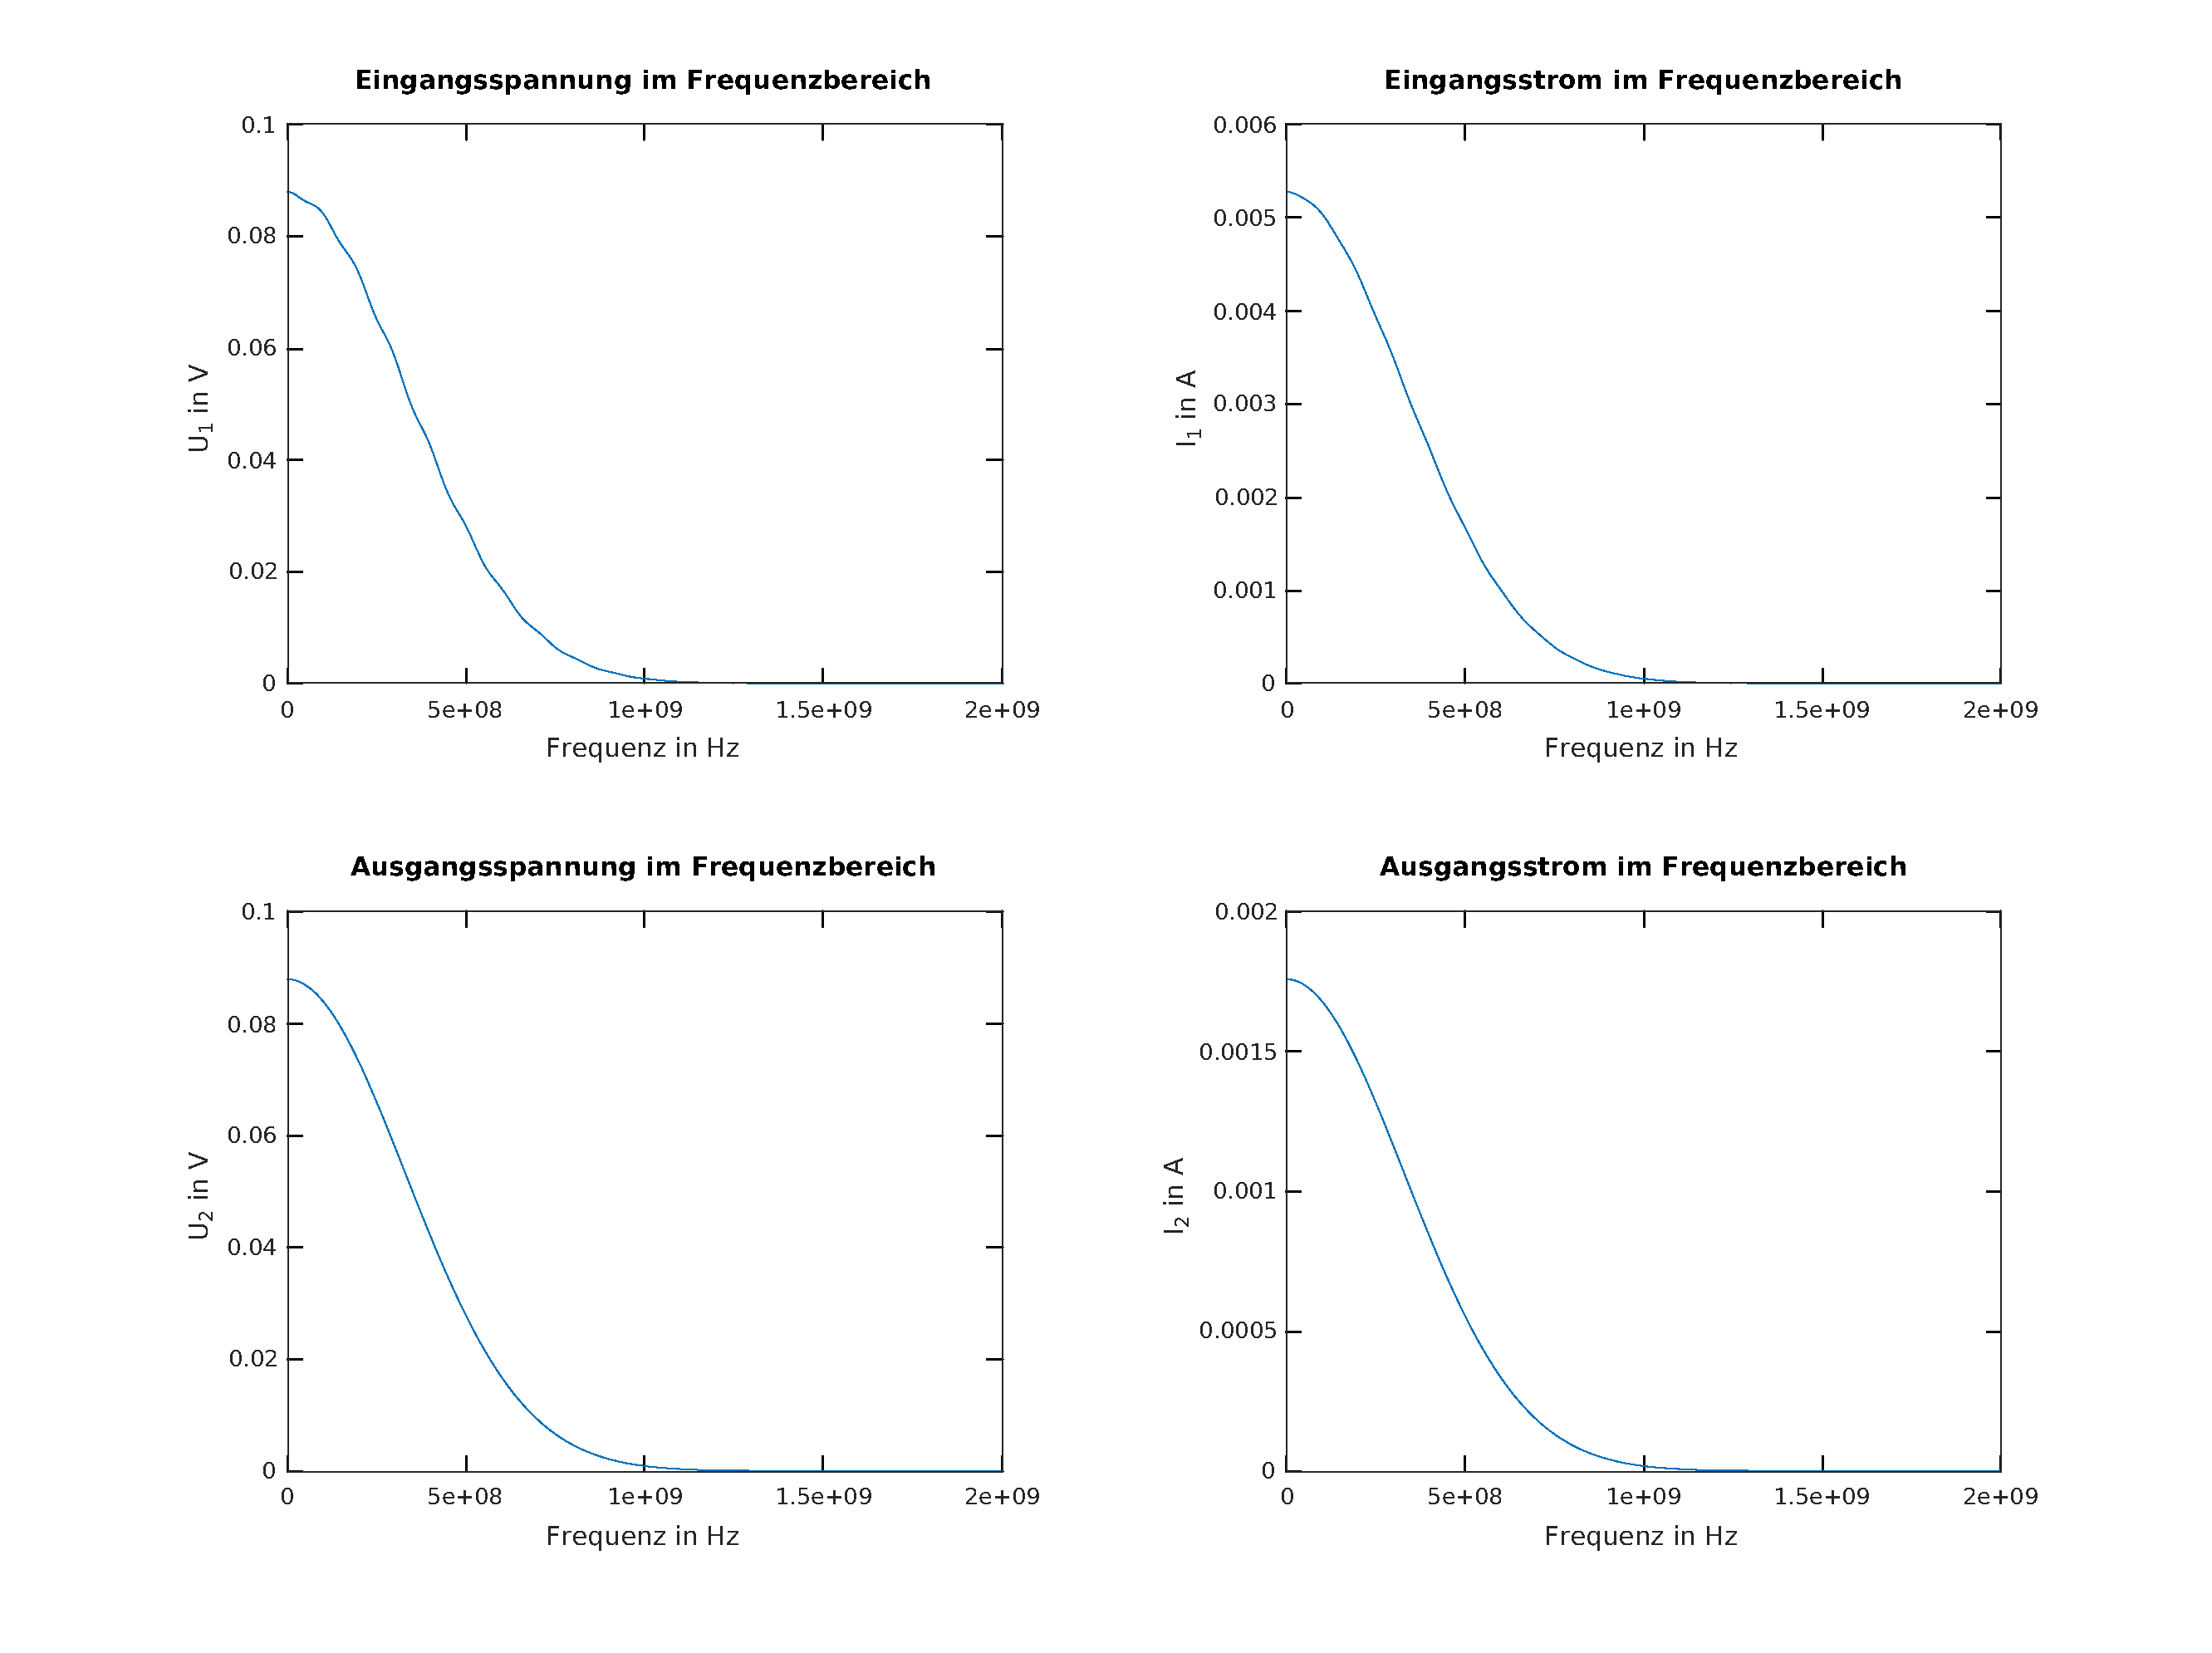
\includegraphics[width=0.9\linewidth]{EinAusSpanStromFrequenz}
	\caption{Ein- und Ausgangsspannungen  und Ströme der homogenen Koaxialleitung im Frequenzbereich}
	\label{fig:einausspanstromfrequenz}
\end{figure}

% --> Aufgabe
\begin{framed}
	\noindent \textbf{5.} Berechnen Sie die Ein- und Ausgangsimpedanz im Frequenzbereich und stellen 
Sie diese in Abhängigkeit der Frequenz dar.\label{exer:ZfreqDomain}
\end{framed}
\noindent
Im Frequenzbereich verhalten sich die Ein- und Ausgangsimpedanzen wie in den Abb. \ref{fig:eingangsimpedanz} und \ref{fig:ausgangsimpedanz} dargestellt. Es ist deutlich zu erkennen, dass die Ausgangsimpedanz, wie angesetzt dauerhaft bei 50\, Ohm liegt
\begin{figure}
	\centering
	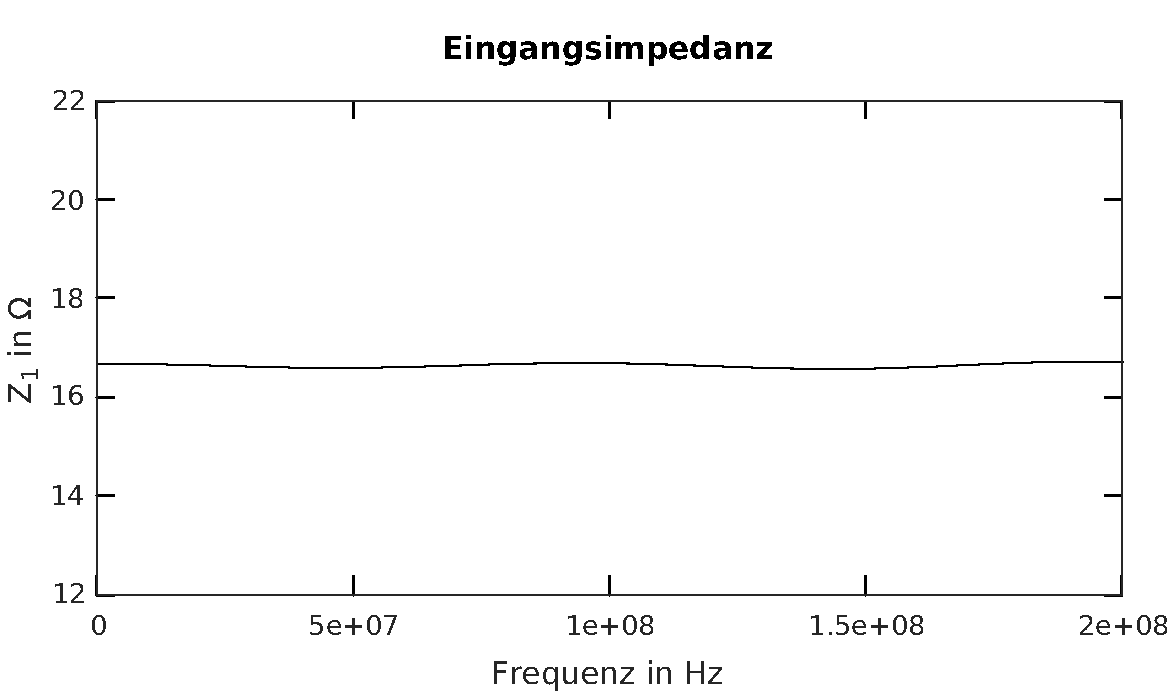
\includegraphics[width=0.7\linewidth]{Eingangsimpedanz}
	\caption{Eingangsimpedanz im Frequenzbereich für die homogene Koaxialleitung}
	\label{fig:eingangsimpedanz}
\end{figure}

\begin{figure}
	\centering
	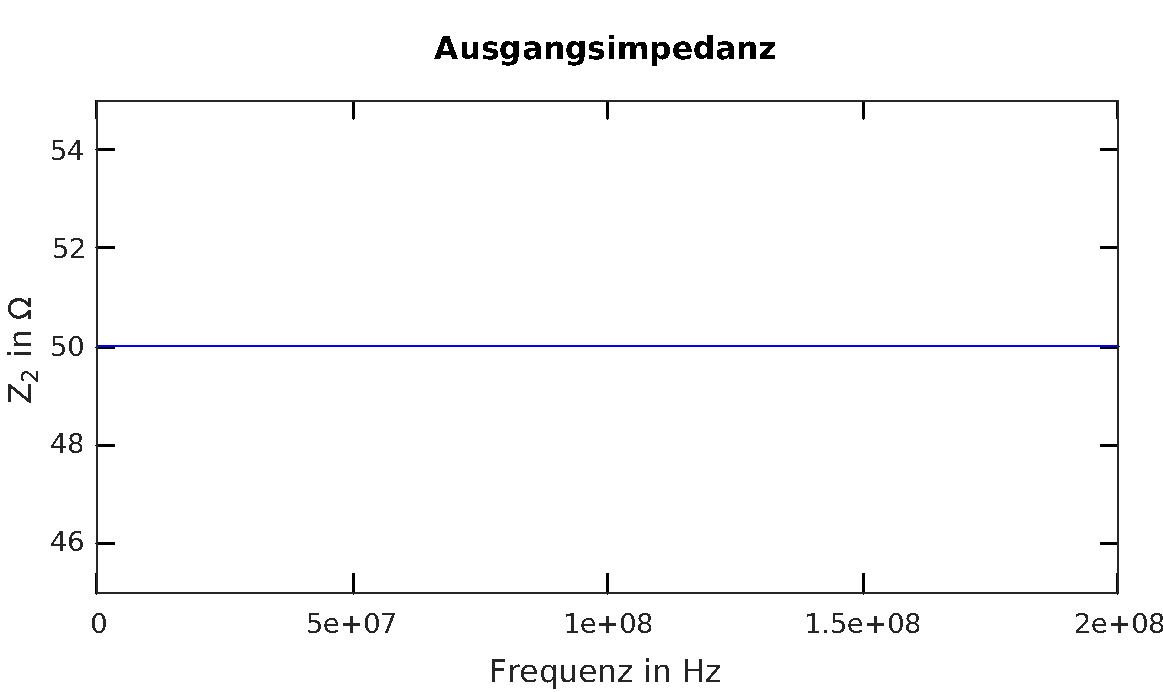
\includegraphics[width=0.7\linewidth]{Ausgangsimpedanz}
	\caption{Ausgangsimpedanz im Frequenzbereich für die homogene Koaxialleitung}
	\label{fig:ausgangsimpedanz}
\end{figure}

% --> Aufgabe
\begin{framed}
	\noindent \textbf{6.} Berechnen Sie aus den Spektren der Strom- und 
Spannungsgrößen die Spektren der zugehörigen Wellengrößen $a_1$,
$b_1$ und $b_2$ und daraus die Streuparameter $S_{11}$ und
$S_{21}$. Interpretieren Sie das Ergebnis für Reflexion und
Transmission.\label{exer:calcWaveQuantities}
\end{framed}
\noindent
Die Streuparameter beschreiben verschiedene Reflexions und Transmissionseigenschaften. $S_{11}$ beschreibt den Eingangs-Reflexionsfaktor, $S_{21}$ den Vorwärts-Transmissionsfaktor. Sie sind ein Maß dafür, wie stark am Eingang auftreffende reflektierte Wellen reflektiert oder transmittiert werden. Aus Abbildung \ref{fig:sparameterenergie} ist zu entnehmen, dass diese Parameter nicht stark von der Frequenz abhängig sind.

\begin{figure}
	\centering
	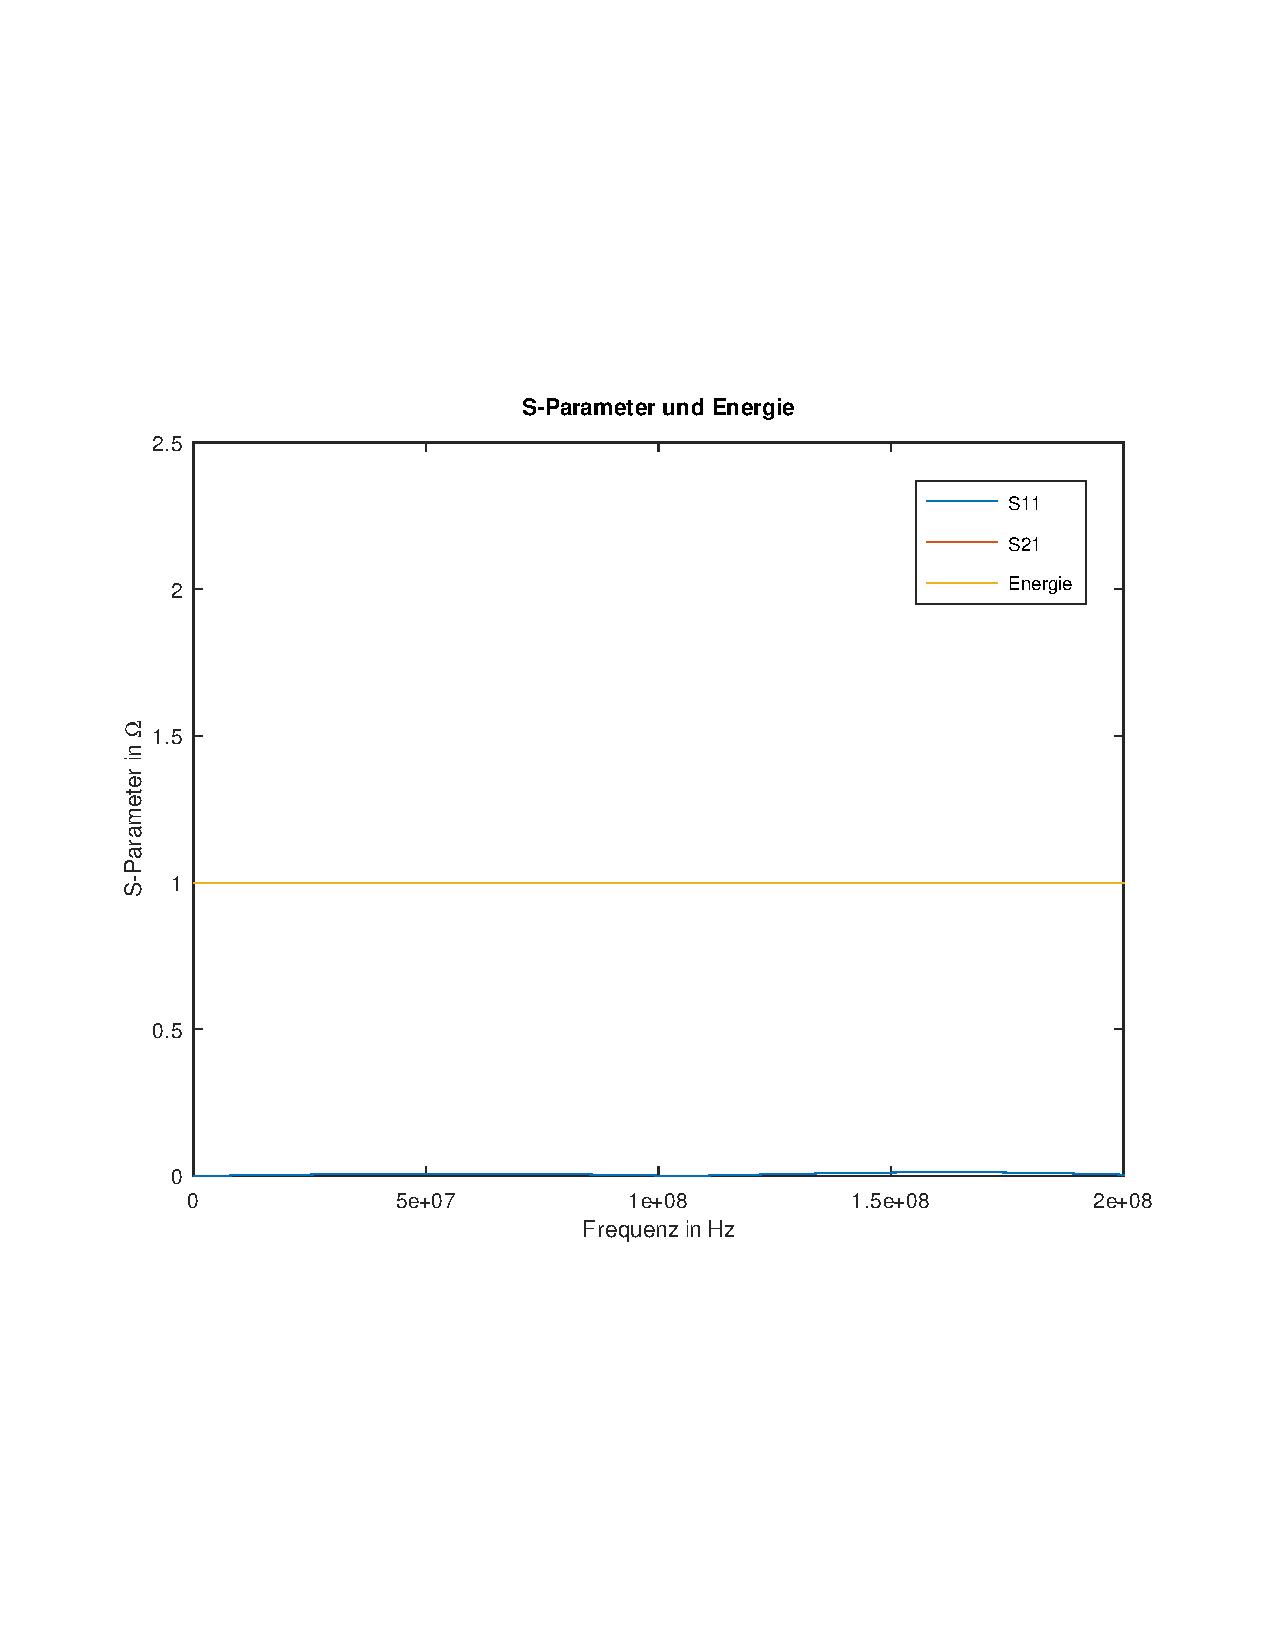
\includegraphics[width=0.7\linewidth]{SParameterEnergie}
	\caption{Spektren der Streuparameter $S_{11}$ und $S_{21}$ sowie die Energiebilanz $|S_{11}|^2 + |S_{21}|^2$ im homogenen Fall}
	\label{fig:sparameterenergie}
\end{figure}


% --> Aufgabe
\begin{framed}
	\noindent \textbf{7.} Überprüfen Sie die Energiebilanz nach~(8.8).\label{exer:checkEnergyBal4TLine}
\end{framed}
\noindent
Bei unserer Untersuchung der Energiebilanz kommen wir auf eine Energiebilanz von 5 was auf einen Fehler in der Implementierung oder Rechenvorschrift hindeutet, den wir aber nicht zu finden in der Lage waren. Diese Annahme ist vor allem dadurch begründet, das die anderen Ergebnisse der Berechnungen sich im erwarteten Ergebnisbereich befinden, was bei dieser Energiebilanz so nicht sein könnte. 

% --> Aufgabe
\begin{framed}
	\noindent \textbf{8.} Wiederholen Sie die Berechnungen für die inhomogene Leitung.\label{exer:calc4inhomTLine}
\end{framed}
\noindent
Aus \ref{fig:inhomo_1} ist zu erkennen, dass im inhomogenen Fall Reflexionen auftreten. Diese sind sowohl am Eingang, aber auch am Ausgang messbar. Die Reflexionen entstehen durch die Inhomogenität der Leitung und den damit verbundenen Reflexions- und Transmissionsparametern.\\
\\
In Abbildung \ref{fig:inhomo_2} ist nun ein anderes Frequenzsprektrum, als im homogenen Fall. Dies liegt an den gerade beschriebenen Reflexionen, die andere Frequenzanteile enthalten, als der Ausgangspuls. Die Anforderung eines begrenzten Signals im Frequenzbereich ist aber weiterhin erfüllt.\\
\\
Bei der Eingangsimpedanz, die in Abbildung \ref{fig:inhomo_3} dargestellt ist, ist nun eine deutlich höhere Frequenzabhängigkeit erkennbar, als im homogenen Fall. Die Ausgangsimpedanz aus Abbildung \ref{fig:inhomo_4} liegt weiterhin bei den festgesetzten $50\,$Ohm.\\
\\
Auch die Streuparameter und die damit verbundene Energiebilanz aus Abbildung \ref{fig:inhomo_5} zeigen nun eine deutlich höhere Frequenzabhängigkeit als vorher. Dies bedeutet, dass sowohl die Reflexion, als auch die Transmission am Eingang stärker von der Frequenz abhängig sind, als im homogenen Fall.

\begin{figure}
	\centering
	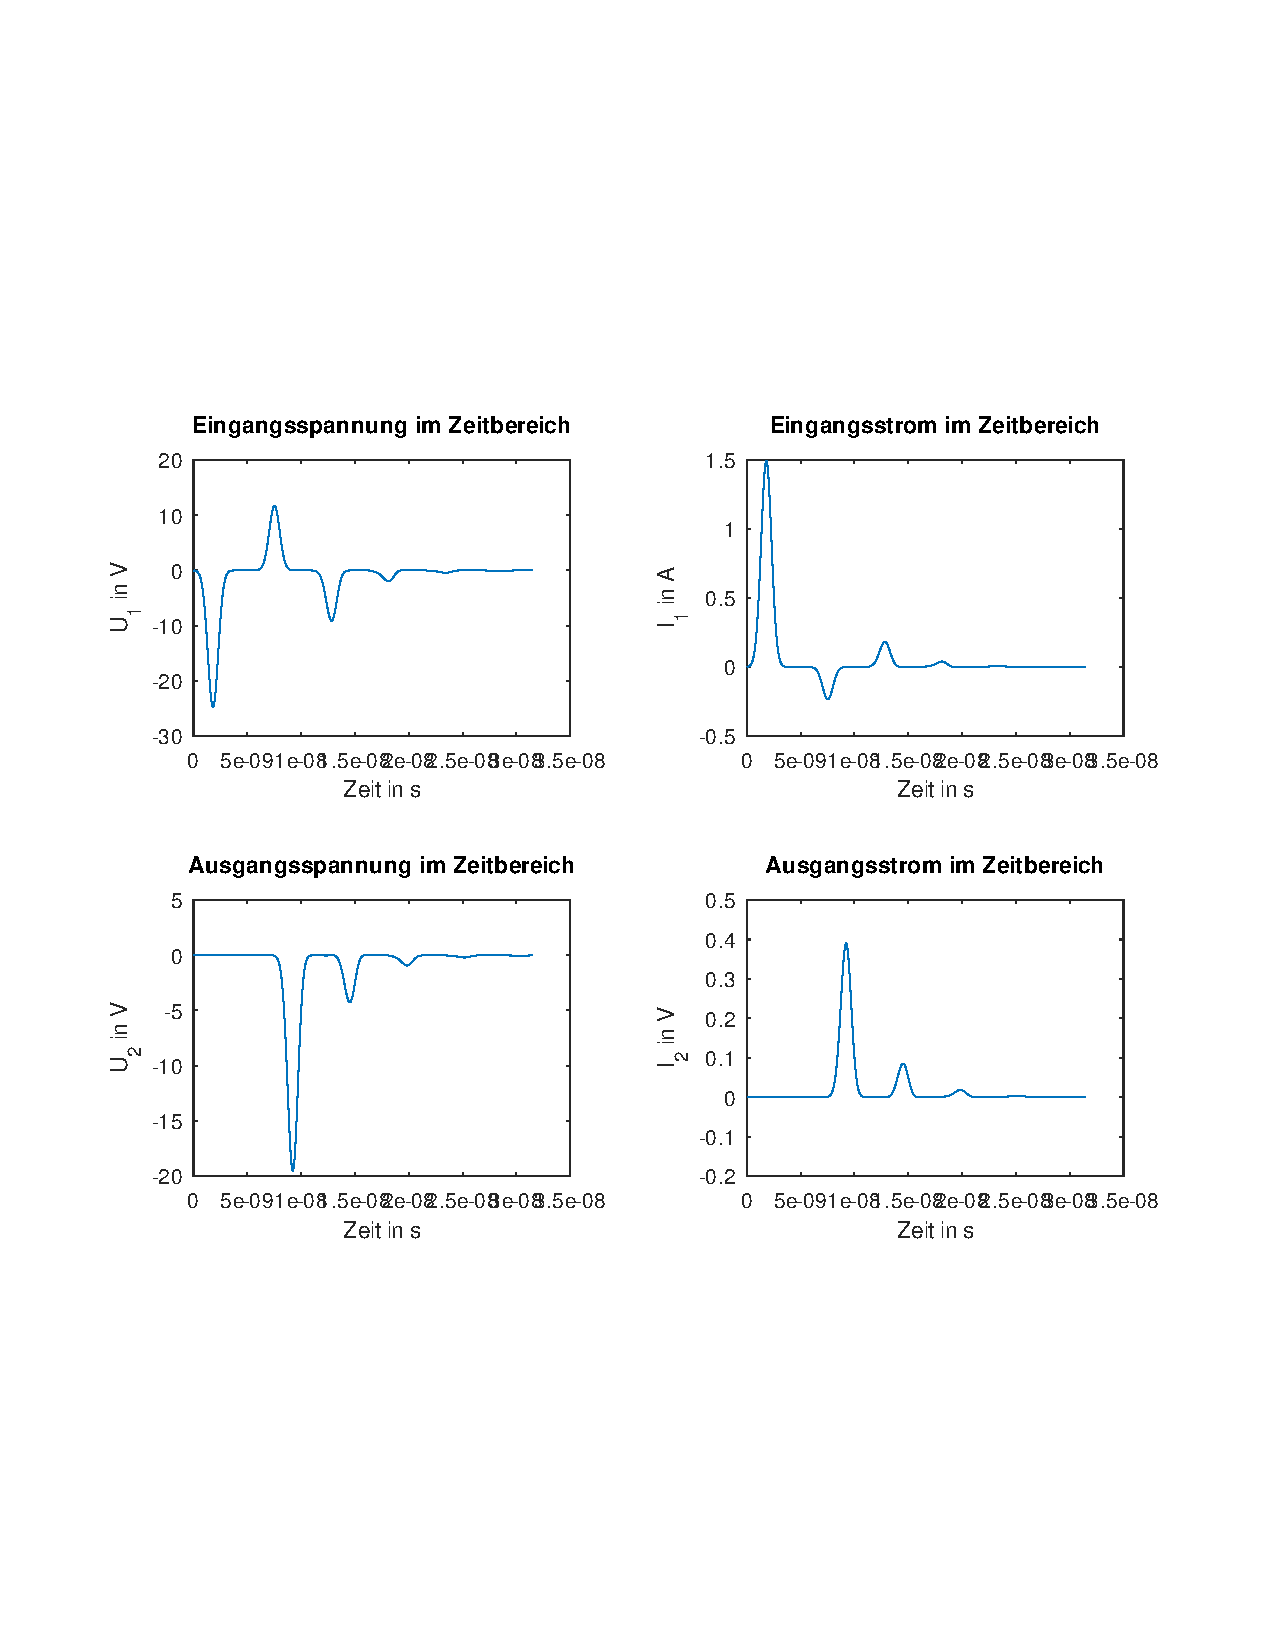
\includegraphics[trim = 15mm 65mm 15mm 65mm, clip,width=0.7\linewidth]{inhomo_12}
	\caption{Ein- und Ausgangsspannungen  und Ströme der inhomogenen Koaxialleitung im Zeitbereich}
	\label{fig:inhomo_1}
\end{figure}
\begin{figure}
	\centering
	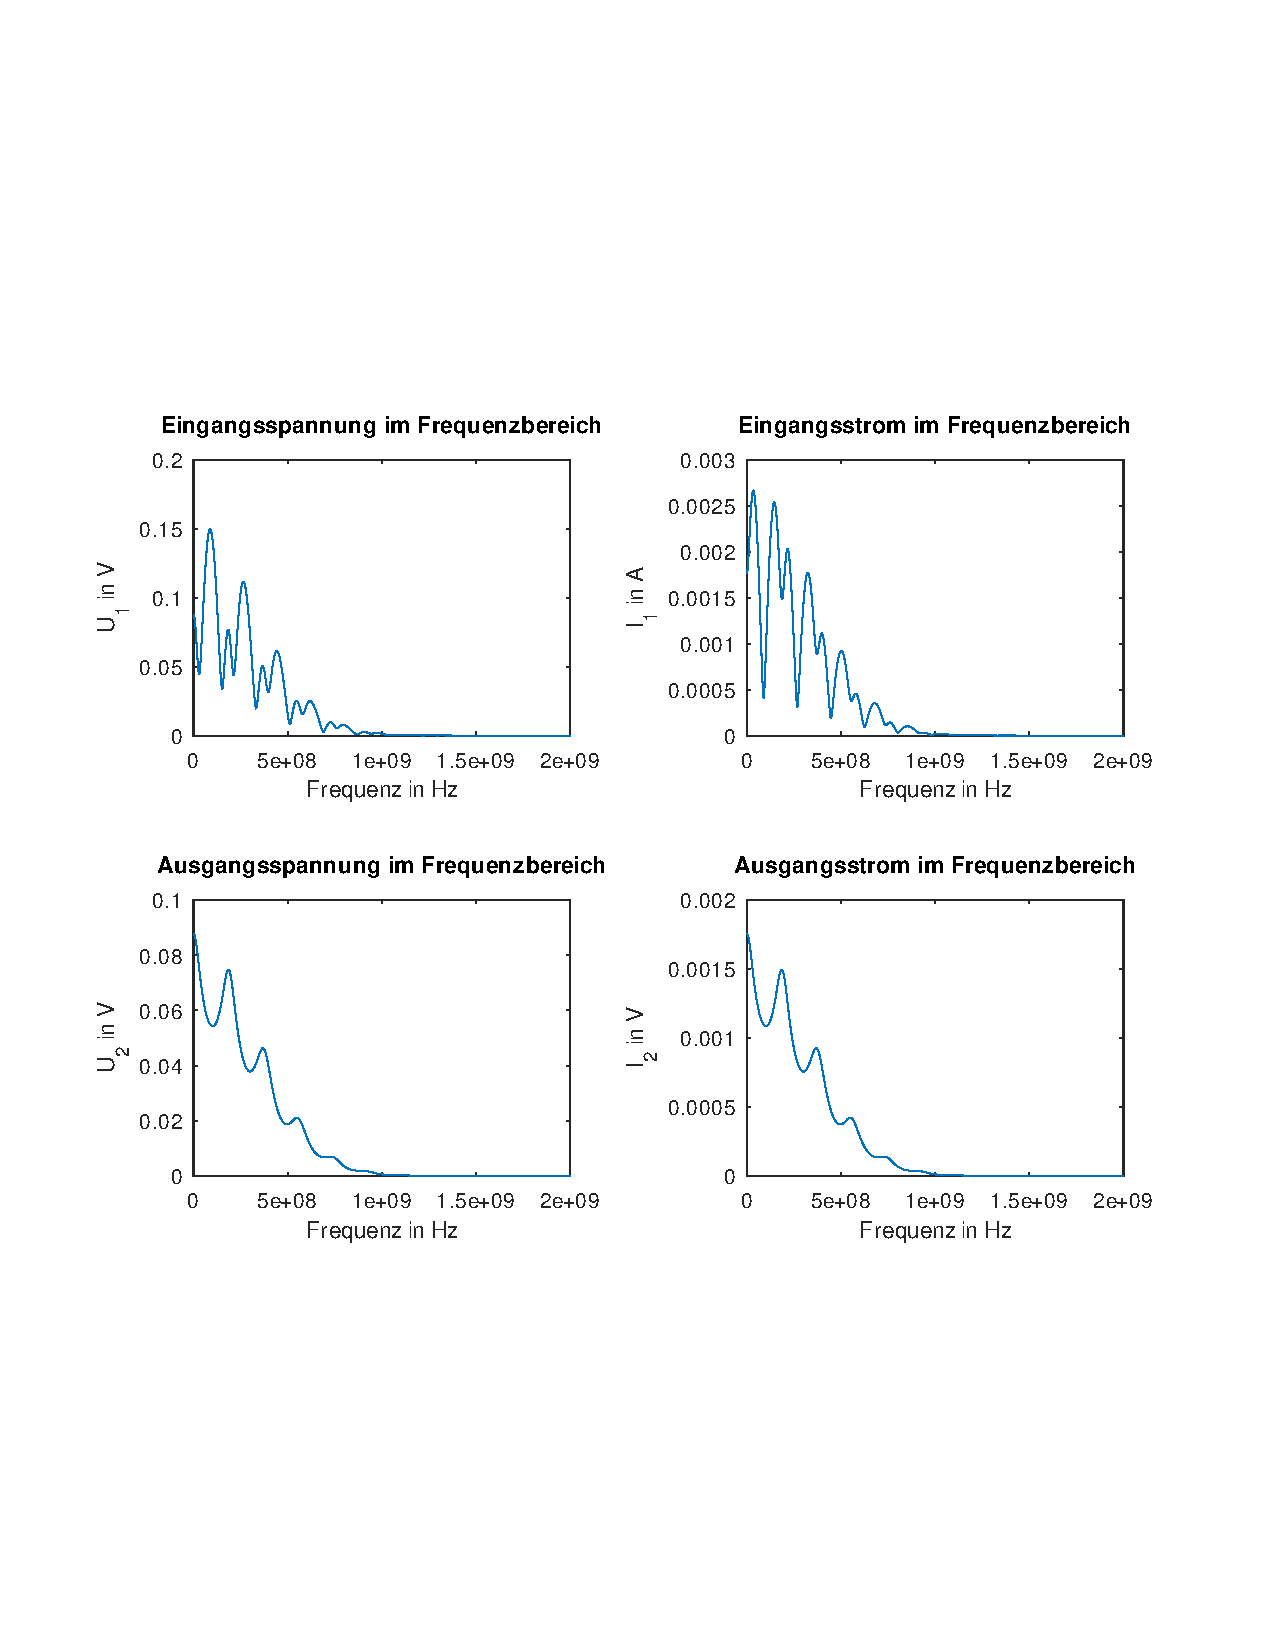
\includegraphics[trim = 15mm 65mm 15mm 65mm, clip,width=0.7\linewidth]{inhomo_2}
	\caption{Ein- und Ausgangsspannungen  und Ströme der inhomogenen Koaxialleitung im Frequenzbereich}
	\label{fig:inhomo_2}
\end{figure}
\begin{figure}
	\centering
	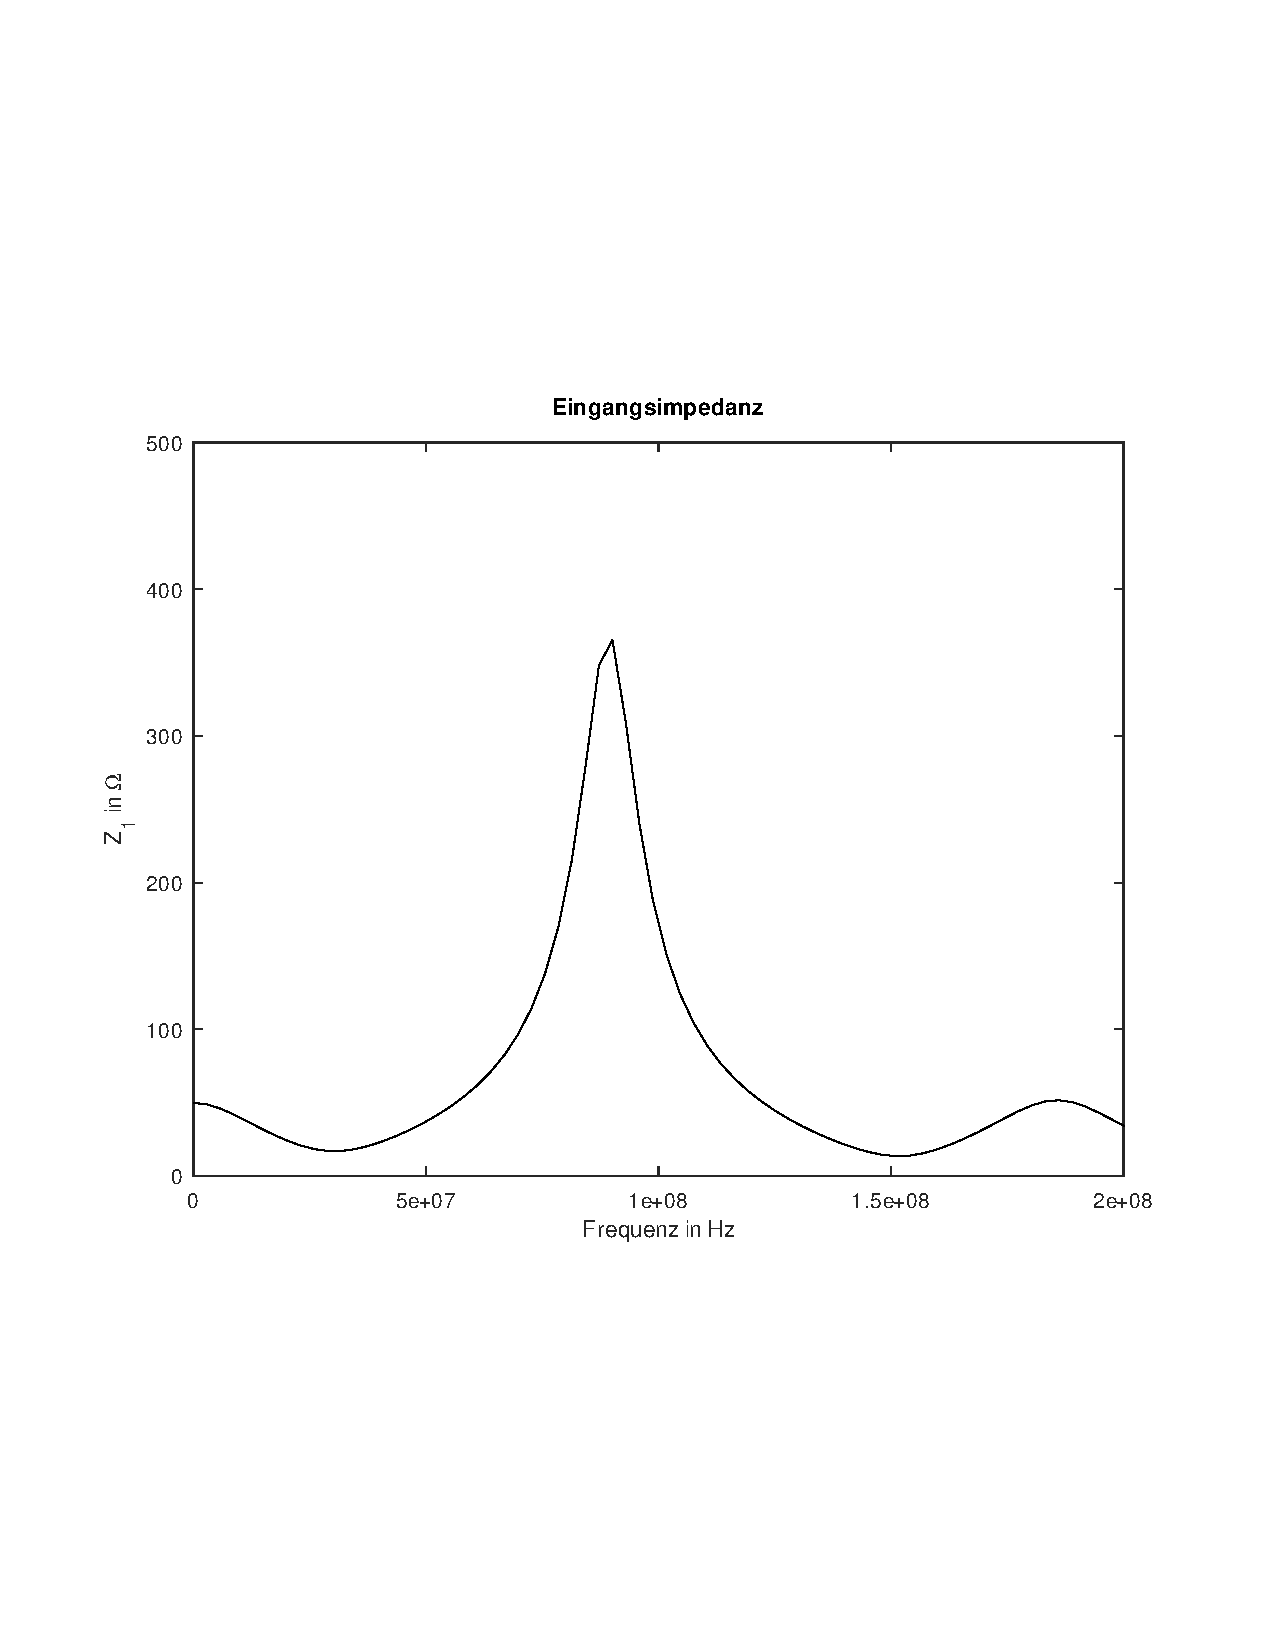
\includegraphics[trim = 15mm 65mm 15mm 65mm, clip,width=0.7\linewidth]{inhomo_3}
	\caption{Eingangsimpedanz im Frequenzbereich für die inhomogene Koaxialleitung}
	\label{fig:inhomo_3}
\end{figure}
\begin{figure}
	\centering
	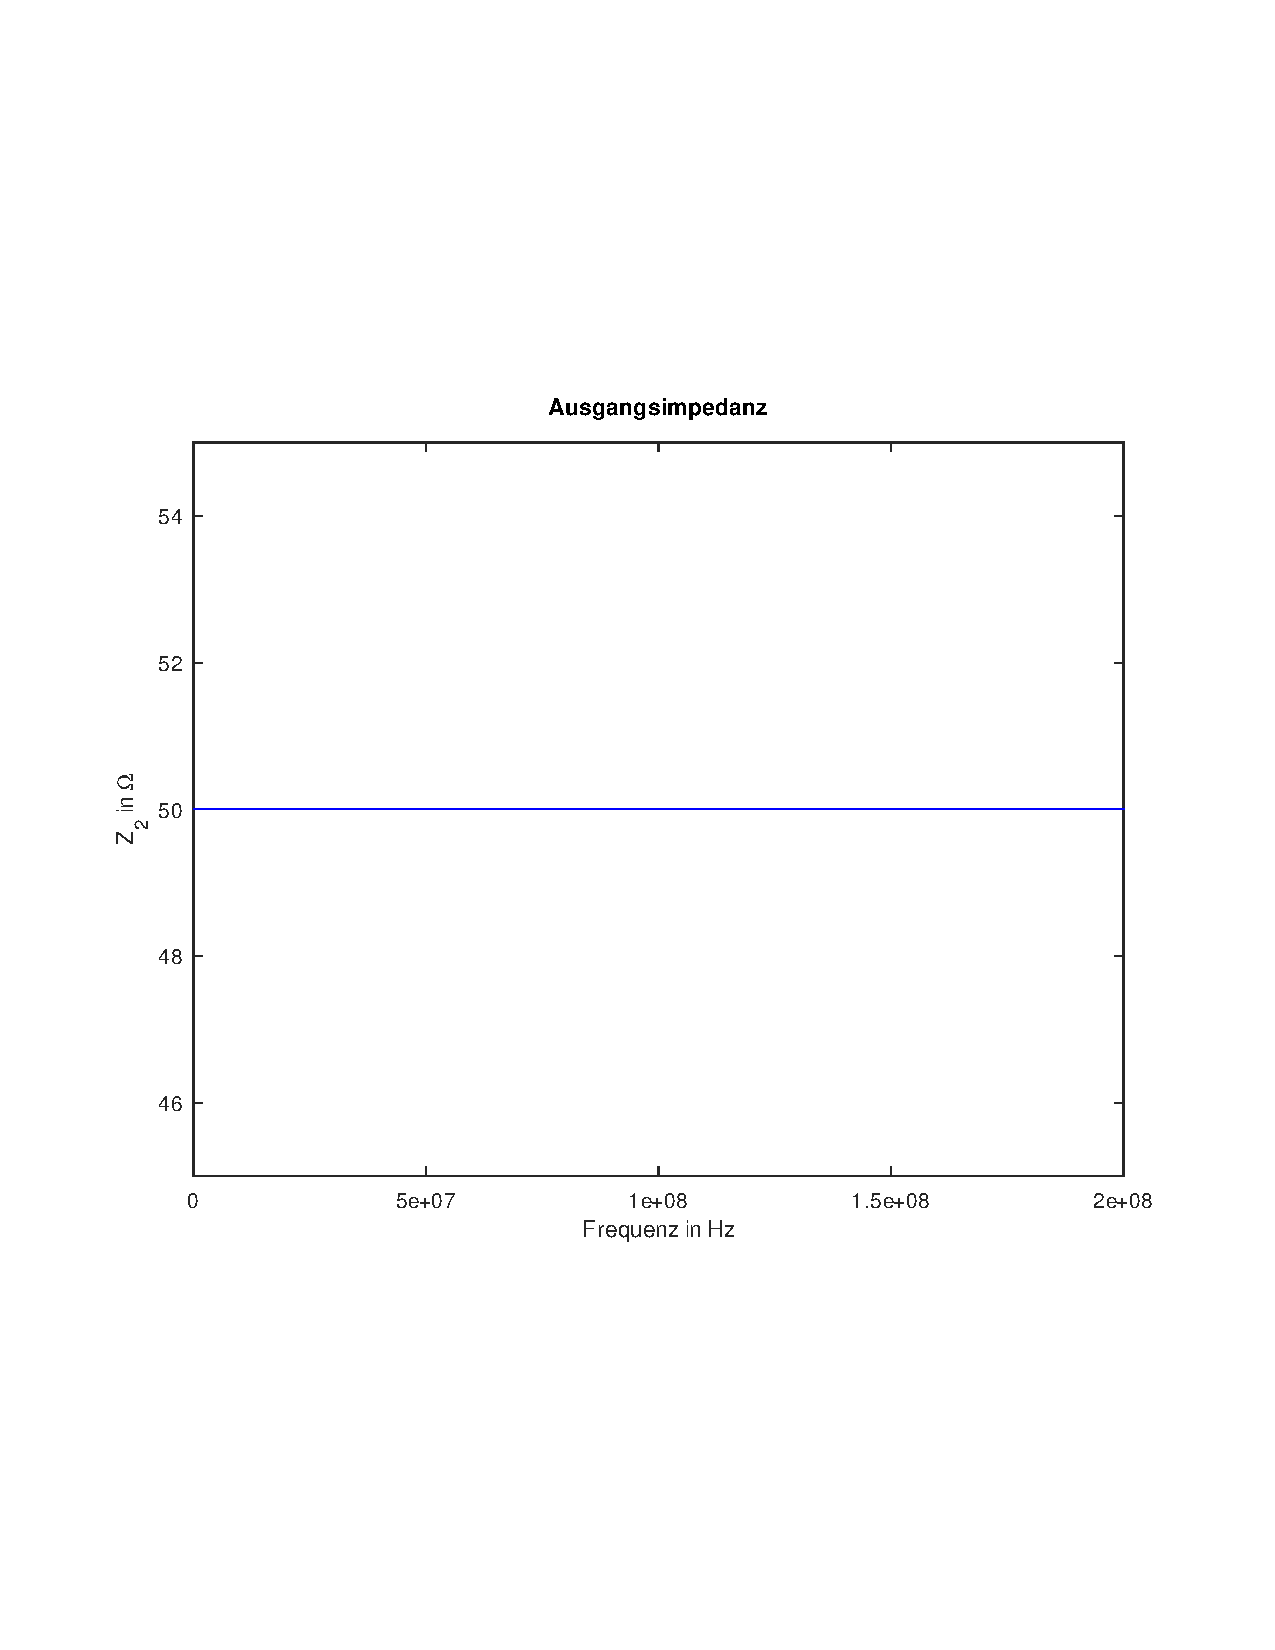
\includegraphics[trim = 15mm 65mm 15mm 65mm, clip,width=0.7\linewidth]{inhomo_4}
	\caption{Ausgangsimpedanz im Frequenzbereich für die inhomogene Koaxialleitung}
	\label{fig:inhomo_4}
\end{figure}
\begin{figure}
	\centering
	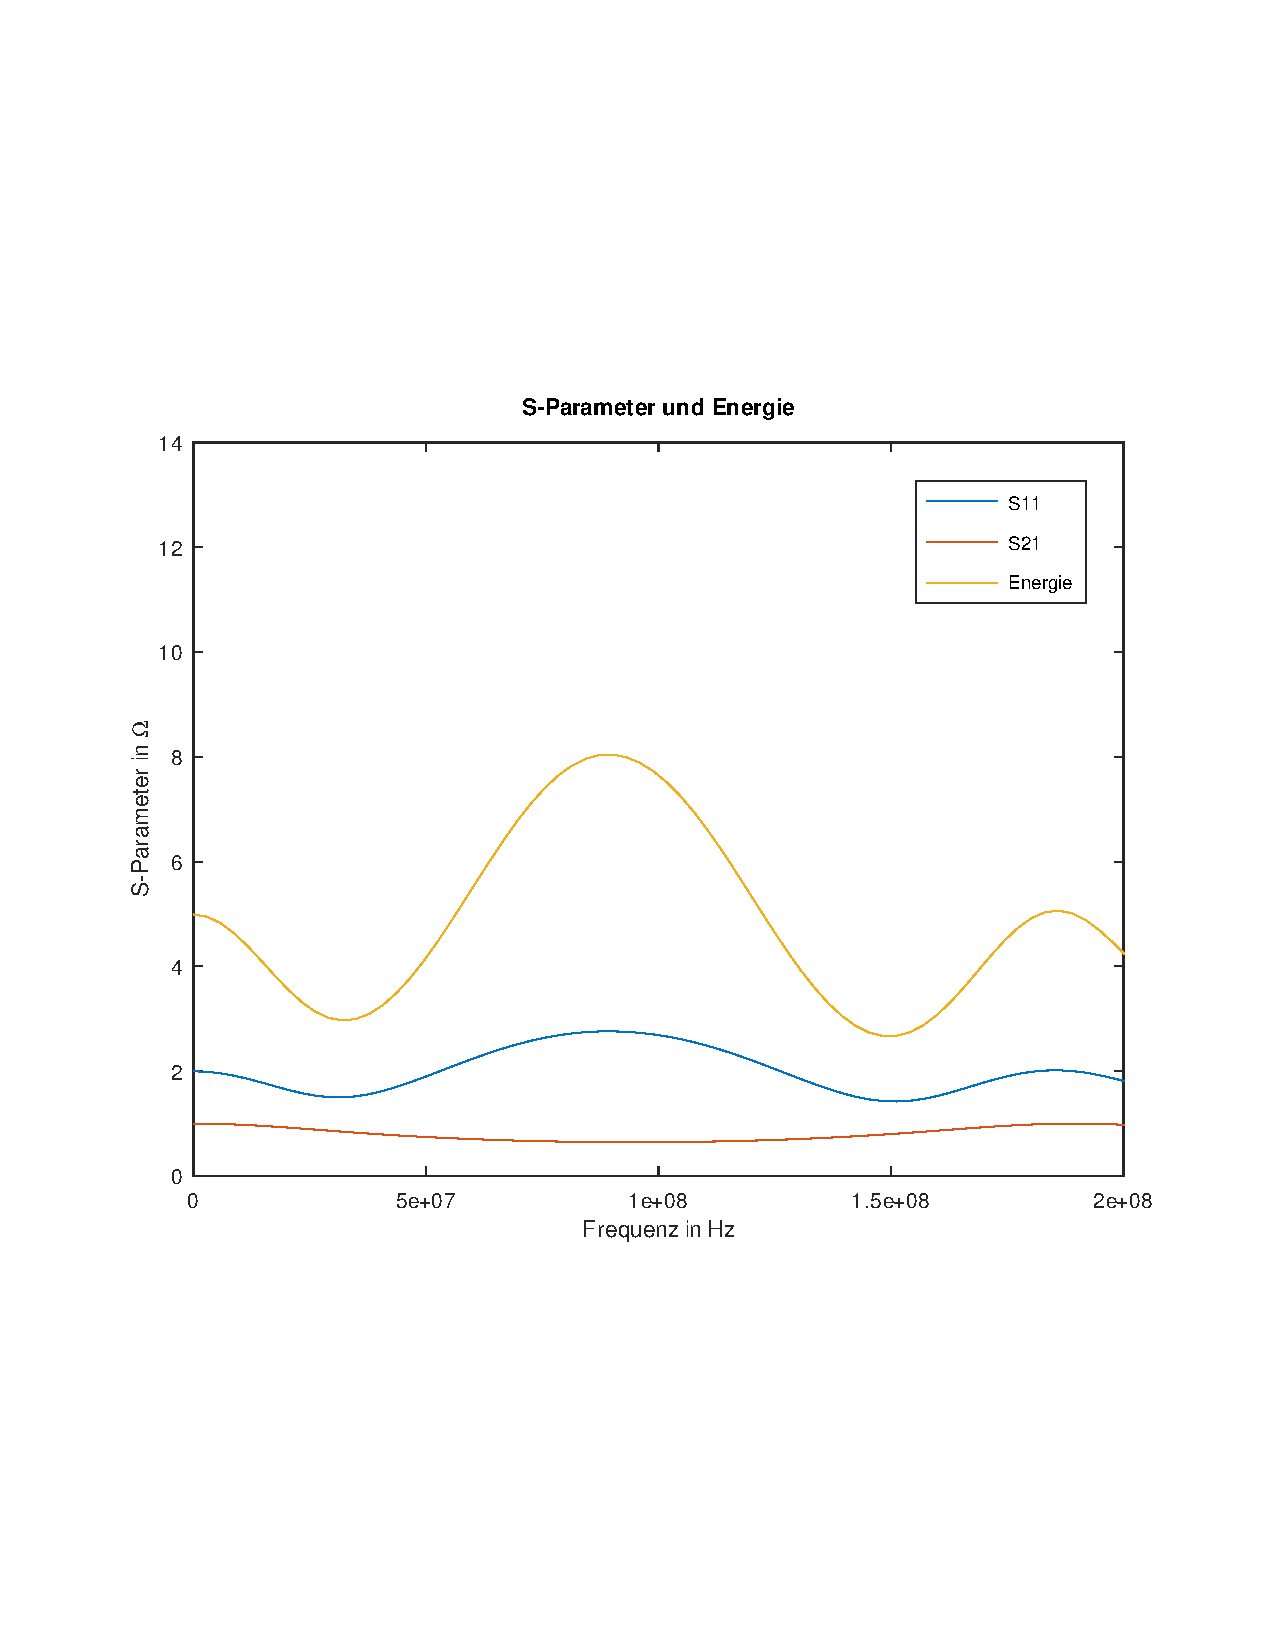
\includegraphics[trim = 15mm 65mm 15mm 65mm, clip,width=0.7\linewidth]{inhomo_5}
	\caption{Spektren der Streuparameter $S_{11}$ und $S_{21}$ sowie die Energiebilanz $|S_{11}|^2 + |S_{21}|^2$ im inhomogenen Fall}
	\label{fig:inhomo_5}
\end{figure}

{\subsection{Lösung im Frequenzbereich}}

% --> Aufgabe
\begin{framed}
	\noindent \textbf{9.} Berechnen Sie das System für einen Frequenzpunkt im
Frequenzbereich, wie in Versuch 5 beschrieben. Die zugehörige
Gleichung für den verlustlosen Fall mit konzentrierten
Elementen lautet
\begin{equation}
	\underbrace{(\curldfit \Mmui \curlfit -
	\omega^2 \Meps + j \omega {\textbf{R}}^{-1} )}_{\Amat} \ul \efit = - j \omega \ul \jfit_{\text{e}}.
\end{equation}
Vergleichen Sie die Rechenzeit dieses einen Punktes mit einem
kompletten Leapfrog-Durchlauf.\label{exer:cmpFreqSolWithLeapfrog}
\end{framed}


\section{Fazit}
Durch die durchgeführten Simulationen ist es nun möglich das Frequenzspektrum eines Signals zu analysieren, sowie Ein- und Ausgangsimpedanz abhängig von der Frequenz zu bestimmen.

\end{document}
